\RequirePackage{ifpdf}
	\ifpdf	
		\documentclass[pdftex]{article}
		\RequirePackage{color} 
	\else
		\documentclass[10pt]{article} 
		\usepackage{nohyperref}		
	\fi

\usepackage[utf8]{inputenc}
\usepackage[T1]{fontenc}
\usepackage[left=1.5cm, top=1.3cm, textwidth=18.6cm, textheight=27cm]{geometry}
\geometry{paper=a4paper}
\usepackage{graphicx}
\usepackage{titling}
\usepackage{abstract}
\usepackage{fancyhdr}

\lhead{} \chead{} \rhead{}
\lfoot{\emph{Research Skills and Methodology, 2014/2015}} \cfoot{} \rfoot{\thepage}
\renewcommand{\headrulewidth}{0pt}
\renewcommand{\footrulewidth}{0.4pt}
\pagestyle{fancy}

\posttitle{\par\end{center}}
\preauthor{\begin{center} \large \begin{tabular}[t]{c}}
\postauthor{\end{tabular}\par\end{center}}
\predate{} \postdate{}
\date{}

\pretitle{
\includegraphics[width=.55\textwidth]{eka-pl.png}\par\vspace{1ex}\begin{center}\huge}

\newcommand{\eng}[1]{(ang.\ \emph{#1})}

\title{Metaheuristic Chess Artificial Intelligence}
\author{Maciej Borkowski\\ 195968@student.pwr.edu.pl \and Paweł Pałus\\ 197004@student.pwr.edu.pl  \and Mariusz Waszczyński\\  192660@student.pwr.edu.pl }

\begin{document}
\thispagestyle{empty}
\twocolumn[
	\maketitle
	\begin{abstract}
The use of metaheuristics (ant colony search, genetic algorithm, simulated annealing) in playing the game of chess as one of the players against an external artificial intelligence.
	{
		\begin{description} 
		\item[Index Terms:] \emph{game, chess, metaheuristics, artificial intelligence, ant colony, genetic, simulated annealing, learning, artificial intelligence, AI}
		\end{description}
	}
	\end{abstract}
	\vspace{2em}
]

\section{Introduction}
\label{sec:introduction}

In the age of quickly developing computers there is more and more need for good Artificial Intelligence. A significant number of IT systems tries to appear intelligent one way or another. One of the fields where intelligence appears to be an important factor are multiplayer games played for fun and competitively for hundreds of years. There are numerous methods to imitate an intelligence - neural networks, fuzzy logic, decision trees. Many of the therse methods are being improved upon to this day. Metaheuristics are commonly used to find good, not necessarily optimal solutions for optimization problems and could be used to imitate an real player.

The game of chess drew our attention. It is a game known to most and its rules make for some very complicated strategies thanks to emergent behaviour of the chess system. Worldwide competitions are organized, which verify players skills in this complex game. One of the most important factors in players skills comes from experience - the training. Each chess figure has well-defined moves it is able to take, which results in an astoundingly big number of possible scenarios. A new player quickly finds out that some pieces are more important than others and subconsciously assign to them different weights. It is an important property, which is generally taken into consideration when designing an artificial chess player.~\cite{comparison}

A real chess game is not deterministic from the perspective of one of the players. However, a metaheuristic could be used in this situation to learn from its own mistakes when playing a game of chess, especially when the opponent always uses the same strategy (which is the case when playing with a normal chess AI). The objective of this research is to find out how would metaheuristic algorithms, such as genetic, ant colony search and simulated annealing behave when used as an artificial intelligence in chess.

\section{Optimization Problem}
\label{sec:problem}

The problem describes a standard game of chess, with a square board of 64 fields. Two players have to consecutively move a piece the board onto another field according to complex, well-defined rules. Our task is to find the series of movements in a game of chess that gives the best chance of winning the game in the end. The starting position of pieces can be arbitrary. 

\subsection{Mathematical model}
\label{sec:model}

Given:
\begin{itemize}
 	\item $t \in N$ - initial game turn 
 	\item $n \in N$ - maximum number of game turns intended for playing 
 	\item $i,j \in \{1,2,3,4,5,6,7,8\}$ - number of rows and columns
 	\item $B_{8,8,t}$ - fields on the board taking values $v_{i,j,t}\in R$ describing the field on board (e.g. the chessmen standing on field) during turn t
 	\item f($B_{8,8,t},v_{i,j,t}$) - takes negatives values for bad situations on the field $v_{i,j,t}$ (e.g. an opponent's piece) positive for good situations (e.g. player's piece)
\end{itemize}

To find:

\begin{itemize}
	\item a series of movements starting from $B_{8,8,t}$ and ending in $B_{8,8,t+n}$ according to rules of chess
\end{itemize}

Such that:

\begin{equation}
\label{eq:costfunction}
	\sum_{i,j} f(B_{8,8,t+n},v_{i,j,t+n}) \quad is \quad maximised
\end{equation}


\section{Experimentation system}
\label{sec:project}

\subsection{Chess engine}
\label{sec:engine}

For learning purposes a real, competitive artificial intelligence was required. A choice has been made to use an external chess engine, which provides required functionality. Such engines commonly implement the Universal Chess Interface (UCI)~\cite{uci} for two-way communication between outside application (like the one made for this research) and the engine implementing an artificial intelligence. 
In the end we have chosen to use Firenzina Engine~\cite{firenzina} because of its good implementation of UCI standard and being able to make good moves in a very short amount of time (one milisecond).

From the side of our application the UCI interface had to be implemented, as well as the whole set of chess rules so that human player can know which moves are valid (through graphical cues). Metaheuristics also required this knowledge, because they have to start from making random moves chosen from the set of valid ones. A Graphical User Interface (GUI) was also fully implemented for user's convinience.

\subsection{GUI}
\label{sec:uci}

\begin{figure}[!htb]
	\centering
	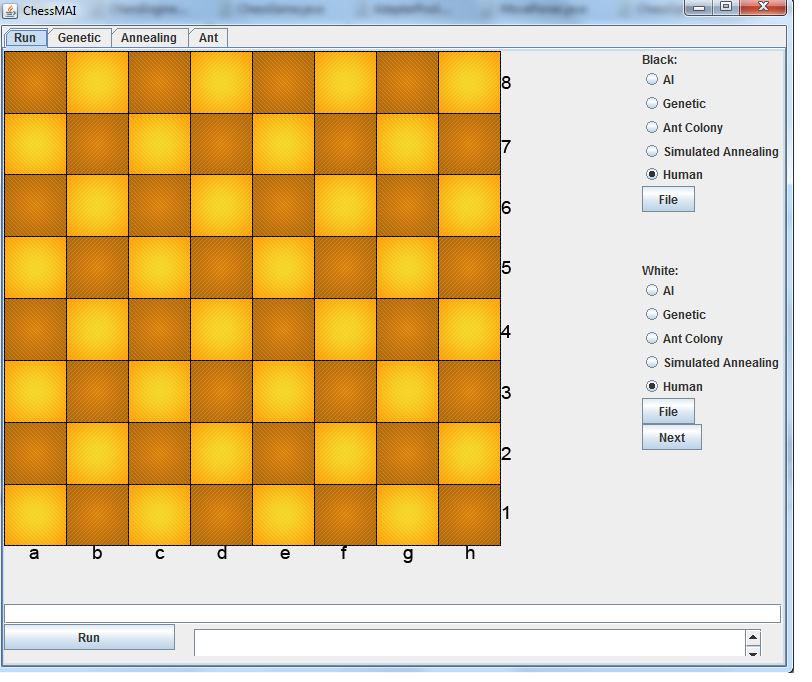
\includegraphics[width=0.5\textwidth]{chessImages/Initial.png} 
	\caption{Initial, empty run panel enables us to choose the types of players and starting game situation}
	\label{fig:initialRunPanel}
\end{figure}

Figure \ref{fig:initialRunPanel} shows run panel that is displayed after starting the application. On the right side of the application the user can see options for white and black player. Checking proper radio button one can choose what type of player will play a game as white player and also as a black player. The choices are: AI (Firenzina engine), human, or one of 3 metaheuristics. There are also File buttons that are used to input knowledge base for ant search algorithm and genetic algorithm (proper file button for proper white or black player), and a Next button that is used to make movements one after another from a textbox that is located in annealing tab. It will be further discussed in a later section. The Next button is not displayed in another figures.

\begin{figure}[!htb]
	\centering
	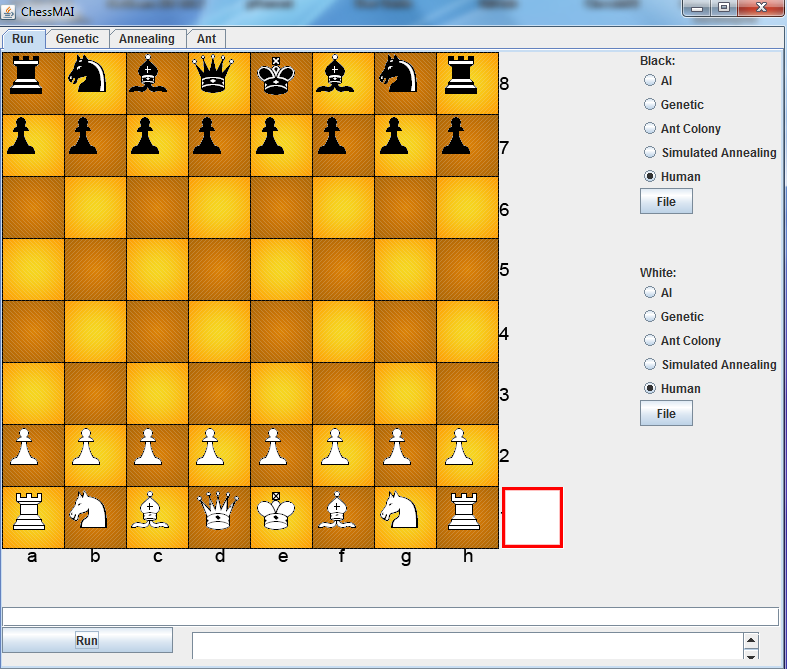
\includegraphics[width=0.5\textwidth]{chessImages/InitialAfterRun.png} 
	\caption{Initial Run panel after pressing run button to start the game}
	\label{fig:initialRunPanelAfterRun}
\end{figure}

Figure \ref{fig:initialRunPanelAfterRun} shows the run panel after pressing the run button. Initial locations of chessmen are set according to chess rules. In the bottom  right corner of the board the is a square coloured black or white depending on which player is expected to make the next move.

\begin{figure}[!htb]
	\centering
	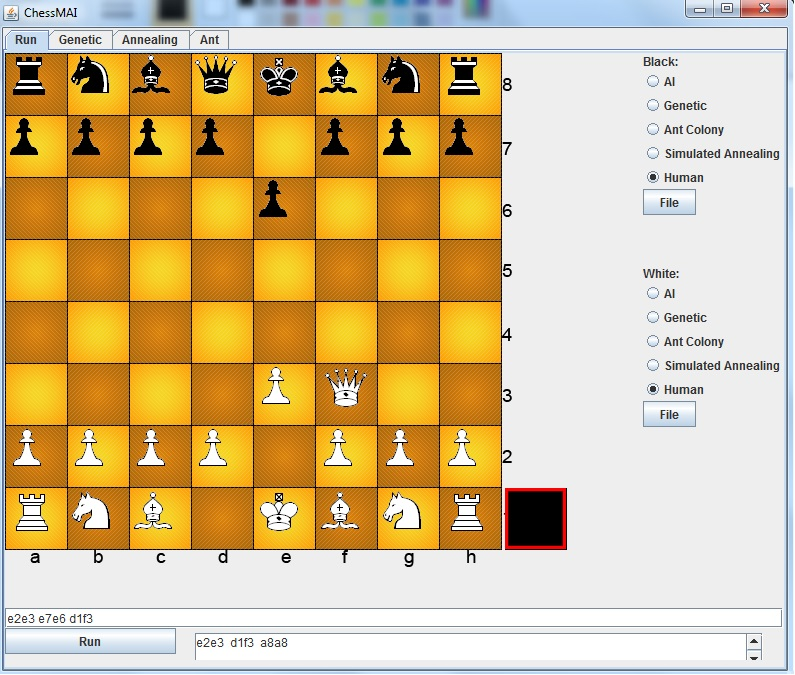
\includegraphics[width=0.5\textwidth]{chessImages/withHistory.png} 
	\caption{Initial board after started with a certain move history}
	\label{fig:runPanelWithHistory}
\end{figure}

The application allows the possibility to start a game from any position other than the standard initial locations of chessmen what is depicted in figure \ref{fig:runPanelWithHistory}. For this purpose sequence of valid movements should be typed (or pasted) to the textbox located above the run button.

\begin{figure}[!htb]
	\centering
	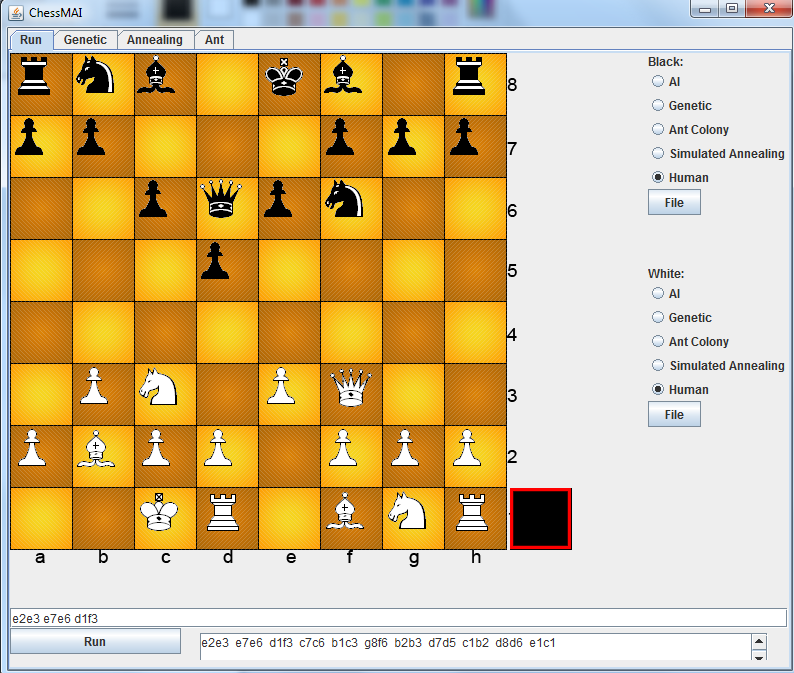
\includegraphics[width=0.5\textwidth]{chessImages/withHistoryAndGameHistory.png} 
	\caption{History of movements}
	\label{fig:runPanelWithMovementsHistory}
\end{figure}

On the right side from the run button one can see the textbox responsible for showing the history of the movements as depicted in figure \ref{fig:runPanelWithMovementsHistory}. This is the full history of movements including movements that was made using the textbox above the run button and its primary use is to copy it into a move history field to always start the game from this position.

At the top of the application are tabs for metaheuristics, where the learning phase can be started, which are will be described in according sections later.

\section{Algorithms}
\label{sec:project}

\subsection{Ant colony (Maciej Borkowski)}
\label{sec:ant}

\subsubsection{Idea}
For ant colony search algorithm a mapping is created between a placement of chess pieces on a chessboard and a list of possible moves the current player is able to do, when provided such board. Each move on this list is additionally annotated with a real value, which describes the fitness of the move. Moves with higher fitness ought to yield us better results. Such mapping is called a pheromone and a set of them pheromones (Figure \ref{fig:pheromones}).

\begin{figure*}[!htb]
	\centering
	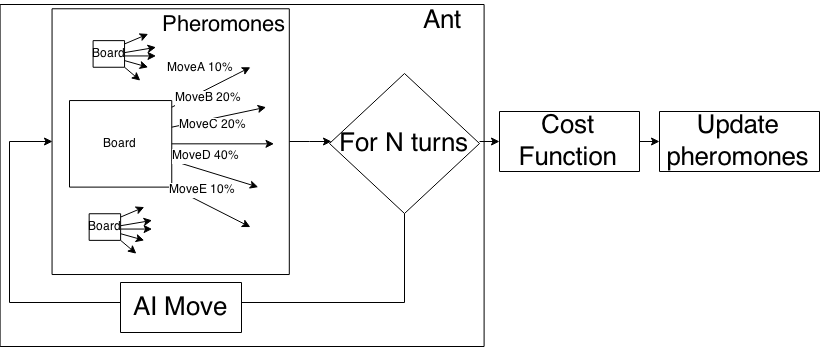
\includegraphics[width=1\textwidth]{ant/pheromones.png} 
	\caption{Diagram of the implemented ant colony search algorithm with visualisation of pheromones for one iteration with one ant}
	\label{fig:pheromones}
\end{figure*}

Ant is defined here as a chess player, that uses pheromones to choose a move when it is metaheuristic's time to make a choice of movement. Ant can be a part of a colony, in which case the colony provides the pheromones or it can be independent (used for Greedy Mode). Pheromones can be saved to and loaded from a file. When an ant finds itself on a board that has not yet been added to pheromones a new pheromone is created (possible moves for the board are computed and assigned equal real values).

 Ant can work in one of two modes: 
\begin{itemize}
 	\item Adventurous Mode \hfill \\
		Used for learning. In this case the ant works for the betterment of its colony. It chooses moves randomly, according to the values of pheromones. This strategy improves the pheromones, by visiting a wide range of possible boards, which results in frequent updates and addition of new pheromones. The probability of choosing move M (with real value v):
\begin{equation}
\label{eq:choosingequation}
	P(M) = \frac{v_m + |min(V)|}{\sum V + n|(min(V))|}
\end{equation}
where~$V$ are all values in a given pheromone,~$v_m$ the value for move and~$n$ is the length of~$V$.

	\item Greedy Mode \hfill \\
		Used for testing and real games. In this case the ant plays for the best end result in its game. Ant chooses a move from the pheromone with the highest value to choose the best move in each turn.
\end{itemize}

The process of learning consists of many iterations of ants in Adventurous Mode working as a colony. Each iteration amounts to a few phases:
\begin{enumerate}
 	\item Start new games and wait for them to end \hfill \\
		Each ant plays one game of chess and remembers all boards it has run across, all moves it has chosen to do and the
the cost function of the series of movements (value of cost function for last board).
	\item Update pheromones \hfill \\
		For each ant the pheromones connected to visited boards are updated by a fraction of the value of cost function of the whole series of movements.
\begin{equation}
	v_{new} = v_{old} + \frac{i}{m} cost
\end{equation}
where~$v_{new}$ is the new value, ~$v_{old}$ is the old value,~$i$ is the index of the movement in this series of movements, ~$m$ is the length of the series of movements and~$cost$ ist the value of cost function.
	\item Dissipate pheromones \hfill \\
		Pheromone for each of the boards that has been visited at least once by any ant in this game is decreased by multiplying the value by a parameter.
\begin{equation}
\label{eq:dissipationequation}
	v_{new} =  v_{old} *  (1 - dissipation)
\end{equation}
where~$v_{new}$ is the new value, ~$v_{old}$ is the old value and~$dissipation$ is a parameter. 
\end{enumerate}

Pheromones can be saved to a file. The file consists of a list of pheromones, which can be used when playing in the Run panel. Each is described with two lines:
\begin{enumerate}
 	\item String representation of a board, left to right, bottom to up, where \# means no chessman, upper case letters mean white chessmen and lower case letters mean black chessmen \hfill \\
	\item A list of moves. Each move is described by five integer values. First two are the coordinates of chessman to move, third and fourth where to move the chessman to, the fifth is a special value used for promotion (when a pawn becomes another chess piece) and the sixth a real value of pheromone describing its effectiveness. \hfill \\
\end{enumerate}

\subsubsection{Experiments}

Firstly, it has to be accentuated that chess is a complex game, the number of possible boards that have to be remembered in pheromones is huge and for each ant move another move has to be done by external Artificial Intelligence. Because of these reasons the learning phase of this metaheuristic takes a very long time. To get results appearing significantly different from completely random ones, hours have to be spent on learning. This makes it very difficult and time-consuming to experiment with parameters properly.

\begin{figure}[!htb]
	\centering
	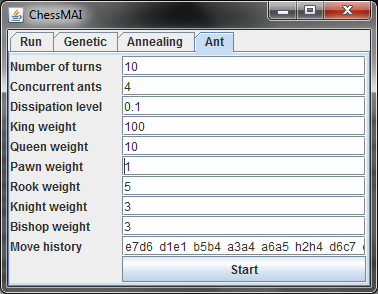
\includegraphics[width=0.5\textwidth]{ant/antapplication.png} 
	\caption{Ant colony dialog boxes}
	\label{fig:antapplication}
\end{figure}

For the experiments the parametrization of many ant search specific variables has been put into dialog boxes in the application(Figure \ref{fig:antapplication}). This way user can change these values easily and create his own colonies. The user-available parameters are as follows:

\begin{itemize}
 	\item Number of turns \hfill \\
The number of turns for each iteration. Each iteration consists of an all concurrent ants playing one game of chance up to a win, lose, draw or the artificial end of game, when it takes too long. This parameter should be kept low if we want the learning phase to take less time and if we want ants to have more broad "knowledge" of possible moves in the beggining of the game. 
	\item Concurrent ants \hfill \\
The number of ants playing a game in each iteration. The more of them the longer each iteration takes.
 	\item Dissipation level \hfill \\
The dissipation parameter of ant search algorithm dissipation equation (Equation~\ref{eq:dissipationequation}).
	\item Piece weight \hfill \\
Each piece has its own weight used in cost function (Equation~\ref{eq:costfunction})
	\item Move history \hfill \\
This parameter sets the starting position of the game from any point, provided a valid chess move history. Each ant in each iteration starts its game from this point and plays up until the end of the game (including the end of maximum number of turns defined as another parameter)
\end{itemize}

The more obvious rules had to be applied to get to the point of metaheuristic being better than a random algorithm and able to win one game out of hundreds when playing against the artificial intelligence. Most importantly the weight of king should far bigger than other figures, the number of turns small, and a move history provided that gives a possibility of winning in a few turns. Increasing the number of concurrent ants and, at the same time, the dissipation level makes the results possibly even better but by a very small margin at the cost of a longer learning phase (making it difficult to test).


\subsubsection{Result}

Meddling in all of these parameters proved to be insufficient in obtaining better results. After careful debugging of the application, the conclusion has been made, that the possible reason for improvement could be to increase the probability of choosing good moves instead of dwell on the bad moves. Even though the move choosing equation (Equation~\ref{eq:choosingequation}) gives more probability to good moves, it is not very significant to the sum of all the probabilities, because there are generally a lot of bad moves. One of the ideas was to sum up the logarithms of values in equation, which is often a way of dealing with those kind of issues. This however only made the values of pheromones more close to each other so the probability of choosing a good move didn't really change that much. 

The really important change was observed when the Equation~\ref{eq:choosingequation} was modified to one with a "tolerance" factor multiplied by each value except the best one. This way the probability of choosing the best move in training is big, enabling  the colony to thoroughly establish how good of a situation on the board it results in. This can quite easily culminate in a fall into a local maximum of cost function, but it is not a bad situation to be in chess - at least we end up in a better situation than before. Additionally to really fall into a local maximum the moves have to contain a lot of weight gain, so it would be most probably a checkmate anyway, which is, for all intents and purposes, a global maximum. Indeed, if a winning sequence of moves has been established in this version the colony started winning very often. At this point a file containing the pheromones could be exported and played in Greedy Mode to win games. 

\subsection{Genetic algorithm (Mariusz Waszczyński)}
\label{sec:genetic}

\subsubsection{Idea}
Our second proposal of a metaheuristic algortihm is the genetic algortihm. It is purely related to how living beings nature evolves through the ages. Looking at it from the perspective of one life beaing equal to one chess game, it may give interesting results. The population consist with many individual living through life - games. The individual is a set of gens which here are called moves. From a programming point of view a mapping is created between a placement of chess pieces on a chessboard and a move for the current player, when provided such board. Each individual is additionally annotated with a real value, which describes the fitness of the final move, calculated with help of cost function (Equation~\ref{eq:costfunction}).

In the application each metaheuristic algorithm works as a set of players. Even Artificial Inteligence is marked as player. Hence different players can play against each other. Genetic player is divided into two modes (similar to the ant colony algorithm's):
\begin{itemize}
 	\item Adventurous Mode \hfill \\
		Used for learning. In this case the individual is created. The moves are chosen randomly.

	\item Greedy Mode \hfill \\
		Used for testing and real games. Based on global individual choosing appropriate moves. If the individual does not recognize current placement of chess pieces on a chessboard, the move is picked randomly.
\end{itemize}

Entire proccess is divided into two phases: generating a population and learning.
Genereting population phase creates a new thread for playing individuals, waits for them to end and updates their fitness.
When the first phase has been finished the learning process which consist of many interations is started.

\begin{figure*}[!htb]
	\centering
	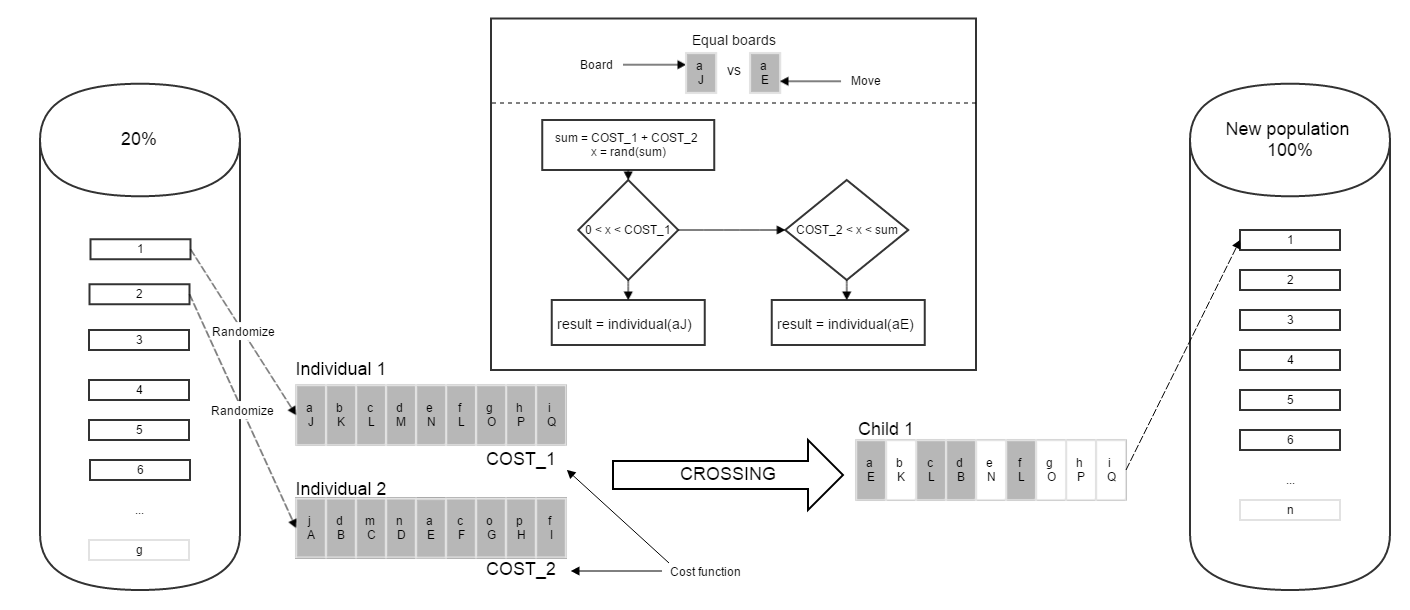
\includegraphics[width=\textwidth]{genetic/genetic_crossing.png} 
	\caption{Genetic: crossing phase}
	\label{fig:genetic_crossing}
\end{figure*}

The iteration has follwing steps:

\begin{enumerate}
 	\item Selection \hfill \\
		The general assume is 80 percent of population have wrong gens and are going to remove (Figure \ref{fig:genetic_selection}).
		
\begin{figure}[!htb]
	\centering
	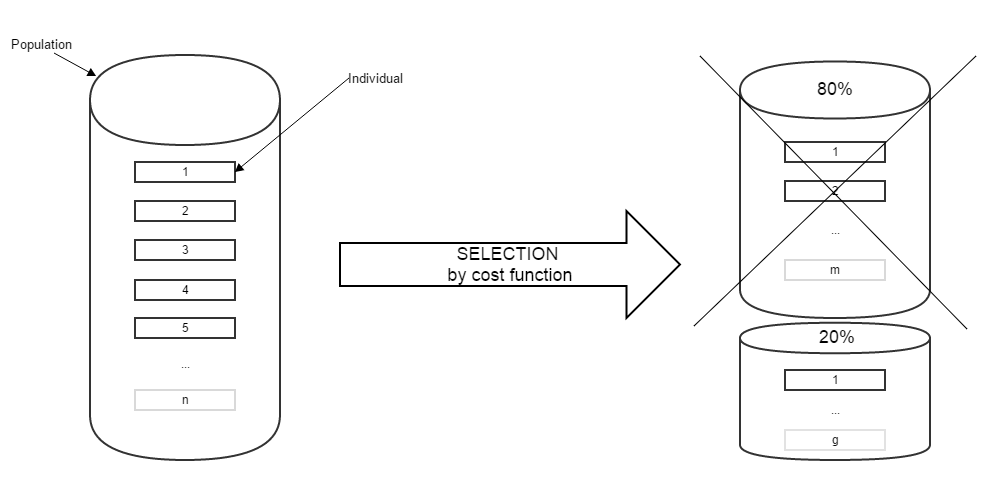
\includegraphics[width=0.5\textwidth]{genetic/genetic_selection.png} 
	\caption{Genetic: selection phase}
	\label{fig:genetic_selection}
\end{figure}

	\item Choosing the global individual \hfill \\
		From the remaining population the individual which has the best cost function is compared with global individual. If it is higher, then global individual is overwritten (Figure \ref{fig:genetic_global}).

\begin{figure}[!htb]
	\centering
	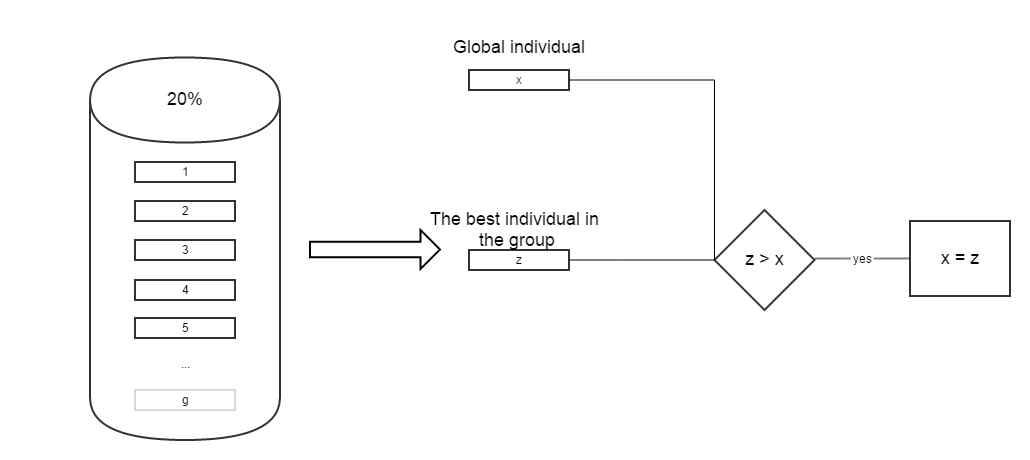
\includegraphics[width=0.5\textwidth]{genetic/genetic_global.png} 
	\caption{Genetic: comparing with the global individual}
	\label{fig:genetic_global}
\end{figure}

	\item Crossing phase \hfill \\
		Two individuals are chosen randomly. Every board\footnote{a placement of chess pieces on a chessboard} from first individual is comparing with every board from second individual. If the boards are equal the proper is chosen and added to the descendant. To choose the optimal one the with not equal probability, cost function are used. Cost function from first and second individual is summed. The sum is a boundary for randomize the number. If the randomized value is from zero to the value of first individual cost function then first individual is chosen, otherwise second individual. Nevertheless if the board has not found an equivalent, it is added to the descendant. Process is showed on Figure \ref{fig:genetic_crossing}. This step is repeating up to fill population, in order to avoid a decrease in population size.

\end{enumerate}

When user decides to stop learning, global individual is stored to file which can be used in normal game - greedy mode.
Optimal time for 5 moves for learning is couple hours.

\subsubsection{Experiment}
\begin{figure}[!htb]
	\centering
	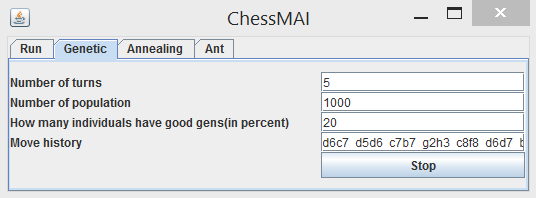
\includegraphics[width=0.5\textwidth]{genetic/genetic_gui.png} 
	\caption{Genetic tab in application}
	\label{fig:genetic_gui}
\end{figure}
In order to play with genetic algorithm, firstly the optimal global individual should be finded. 
The genetic tab is designed for learning purposes. It contains four text fields.

\begin{description}
  \item[Number of turns] \hfill \\
  Determine how many moves the individual have to do. Low value should be used to confine time for learning.
  \item[Number of population] \hfill \\
  Determine size of population.
  \item[How many individuals have good gens] \hfill \\
  Needed for selection phase. Defined 20 percent by default.
  \item[Move history] \hfill \\
  Learning proccess can start from specified board.
\end{description}

Button "start" implies generating population and turning learning proccess on.
Optimal time for learning depends on parameters provided by user. Significant parameters are "Number of turns" and "How many individuals have good gens". First one can minimalize time of learning to achive certain point of knowledge. Second one has direct impact of removing individuals and is associated with "Number of population" parameter. 

\subsubsection{Result}
Unfortunetelly checkmate was not achived. 
For almost 2 thousand tries Artificial Inteligence was winning. The importance of initial board should be emphasized. If cost function is very high at the beginning then is the most probability that genetic algorithm will win. Of course there is a significant impact of the way how cost function is calculated. What factors are takien into consideration, what weight are associated with pieces. 

\subsection{Simulated Annealing (Paweł Pałus)}
\label{sec:annealing}

\subsubsection{Idea}
Simulated annealing is a method for finding a good (not necessarily optimal) solution to an optimization problem.
There are many optimization algorithms, including ant search, genetic algorithms, tabu search, and more. Simulated annealing's advantage is that it avoids getting caught at local minimums solutions that are better than any others nearby, but are not the best.

\begin{figure*}[!htb]
	\centering
	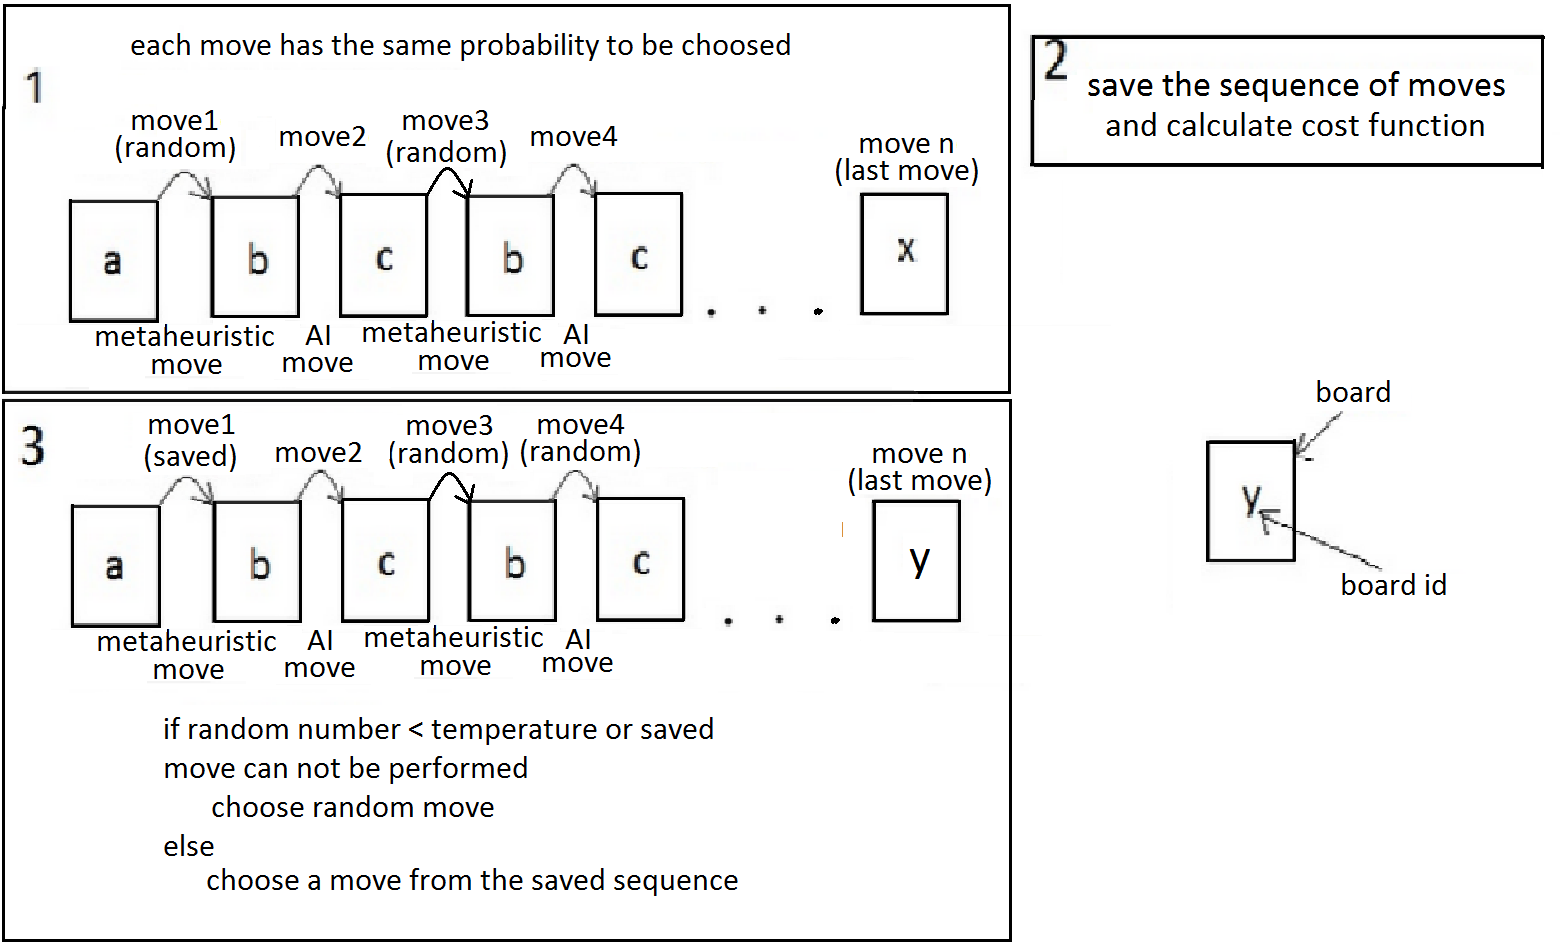
\includegraphics[width=1\textwidth]{annealing/annealingSchema.png} 
	\caption{Diagram of the implemented simululated annealing algorithm}
	\label{fig:annealingSchema}
\end{figure*}

In the first game the Algorithm chooses random possible moves, all moves performed by AI and the algorithm are saved. In the end of the game cost function is calculated and saved. Then the algorithm simulates another game (iteration) in which chooses a saved moves, or a random possible moves and it depends on temperature. If the algorithm has chosen a random move, then the opponent's move is performed by AI, but if saved move was choosed then opponent move is also a saved move. Not always saved move can be performed therefore in case of one cannot make a saved move, a random move is performed. If there is a checkmate or maximum number of turns is achived the game ends and cost function is calculated if this cost function is greater than previous one then old saved moves and cost function are exchanged for present. There can occour a situation in which game ends before achieving maximum number of turns (for example if there is a checkmate) and its cost function is greater than the previous one. Then in the next simulated game the algorithm will have less saved moves for example 4 and when this number is exceeded random moves are performed in metaheuristic's turns and AI moves in opponent turns. The cost function is based only on weights of chess pieces. Weights for chess pieces are as follows:

pawn - 1

knight - 5

bishop - 5

rook - 7

queen - 10

king - 1000

Weights are positive for own pieces and negetive for opponent pieces.
It is important to assign a weight to the king instead of giving weight (in absolute value) value for checkmate, because then it is possible to consider better and worse situations for games that has no max number of turns. without that the algorithm would have all the time the same sequence of saved moves expect very unlikly situation that metaheuristics wins, then the sequence would change only once.

\subsubsection{GUI}
GUI is depicted in figure \ref{fig:annealingTab}).
\begin{figure}[!htb]
	\centering
	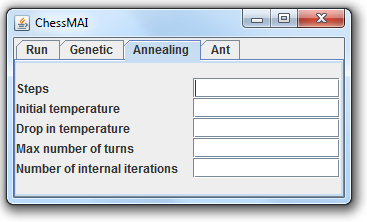
\includegraphics[width=0.5\textwidth]{annealing/GUI.png} 
	\caption{Simulated annealing - dialog boxes}
	\label{fig:annealingTab}
\end{figure}

\begin{itemize}
 	\item Steps \hfill \\
Here is a place to input sequence of moves, after that one can display all or a part of a game in a way that every another move is displayed after pressing  a button

	\item Initial temperature \hfill \\
A decimal number in a range from 0 to 1.0. The greater the temperature the greater the chance of choosing a random move. Temperature decreases after every iteration of algorithm.
 	\item Drop in temperature \hfill \\
A value by which the temperature drops after each iteration.
	\item Max number of turns \hfill \\
An integer number that says how many turns at most can be performed in one game. A turn is defined as two moves, but to simplify number of turns increases after every black player move.
	\item number of internal iterations \hfill \\
An integer number that says how many times the algorithm should repeat an action of searching better solution.
\end{itemize}

\subsubsection{eqperiments}
It is hard to tell what parameters should be used to obtain the best results due to big randomness of the algorithm's work. Some good parameters have been chosen:
\begin{itemize}
	\item Initial temperature = 0.8 \hfill \\

 	\item Drop in temperature = $\frac{Initial \: temperature}{number \: of \: internal \: iterations} \cdot 0.9$ \hfill \\
 	
in this case the temperature for the last iteration equals $10\%$ of the initial temperature. that means $7.2\%$
\end{itemize}
Of course the greater number of the "number of internal iterations" parameter the greater the chance to achieve better solution. Experiments was made in a range from 10 to 20000 for "number of internal iterations" parameter parameter.
Experiments was made most often for value of 10 for "Max number of turns" parameter. There were considered 2 kinds of initial board, standard initial situation for chess and situation depicted in figure 5.

\begin{figure}[!htb]
	\centering
	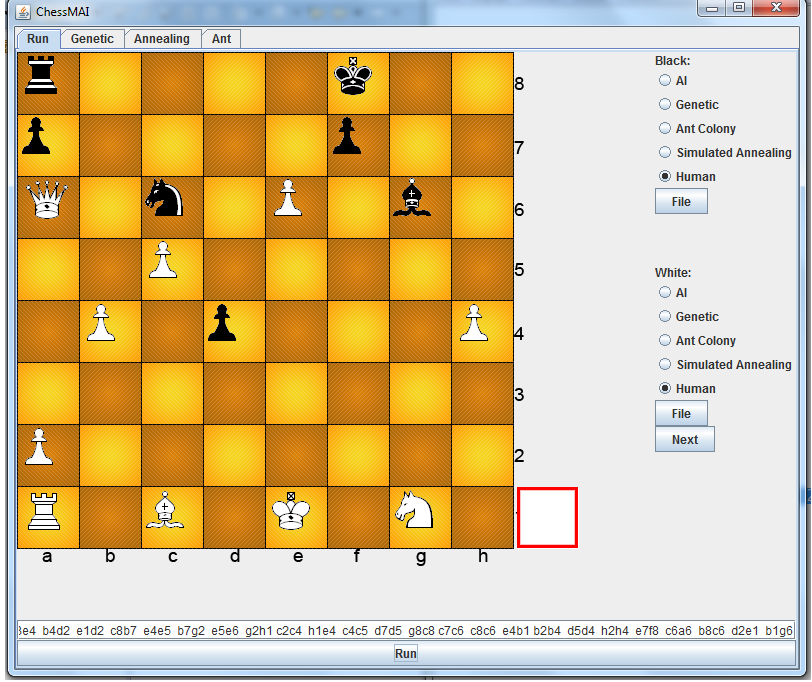
\includegraphics[width=0.5\textwidth]{annealing/board.png} 
	\caption{Initial board}
	\label{fig:initialBoard}
\end{figure}

For above board metaheuristic player is white and it is actually its turn.
 
\subsubsection{Result}
Unfortunetelly checkmate was not achived. The best result for standard initial chess board was cost function: 21.0 for parameters:

- internal iteration number: 10000

- max turn number: 10

- initial temperature: 0.8

- drop in temperature: $\frac{0.8}{10000} \cdot 0.9 = 0.000072$

in time: 1485 seconds

And for initial situation depicted in figure \ref{fig:initialBoard} the best result was cost function equals 31.0 for parameters:

- internal iteration number: 20000

- max turn number: 10

- initial temperature: 0.8

- drop in temperature: $\frac{0.8}{20000} \cdot 0.9 = 0.000031$

in time: 3734 seconds

Different wariants of the algorithm could be considered, the algorithm could simultaneously play for example 5 different games instead of one and at the end of all games choose moves (that would exchange previous saved moves) from the game that achieved the greatest cost function (as far as this cost function would be greater than previous one), or the algorithm could save only its moves and every opponent move would be performed by AI.

It is rare to achive a checkmate by the algorithm due to several precised moves has to be performed to obtain one-time increasing of the cost function. The algorithm would work better if the cost function better expressed a situation on the board. Actually only a material situation is considered, there is a possibility to consider a positional situation, for example the weight of a pawn would increase after each move towards promotion field or the weight of a rook would increase with the number of possible moves that can be performed by the rook, it could be also considered if certain chess piece is protected or not.

\section{Improvements}
\label{sec:improvements}

Some general improvements should be considered for further development of the application:
\begin{itemize}
 	\item Putting all the variables and modes into GUI, so that a wider range of possible parameters can be changed non-programically 
 	\item Adding new engines that implement UCI (other than Firenzina) and use them randomly when choosing a move by AI. This way the metaheuristics will have much wider knowledge. One artificial intelligence can sometimes make mistake moves, but if many engines were to be used randomly, then it would probably not be just a mistake on the part of external AI, but a truly needed sacrifice.
 	\item The learning phases of algorithms are in need of previous data import, so that they can continue learning from a previously saved point.
\end{itemize}

\section{Conclusion}
\label{sec:conclusion}

In conclusion, our experiments proved that it is possible to make a kind of artificial intelligence for chess using metaheuristics that can play better than a completly random algorithm. The results can vary greatly between not only a chosen metaheuristic, but also the chosen parameters and algorithm's details. However, it has to be emphasized that metaheuristics require a huge amount of learning time even when being close to the end of the game and as such would not be viable alternative for a standard type of artificial intelligence.

\begin{thebibliography}{99}

\bibitem{comparison} \textsc{Vecek, N. ; Crepinsek, M. ; Mernik, M. ; Hrncic, D.}, A comparison between different chess rating systems for ranking evolutionary algorithms 
\bibitem{ant} \textsc{Dorigo, M. ; Maniezzo, V. ; Colorni, A.}, Ant system: optimization by a colony of cooperating agents 
\bibitem{genetic} \textsc{David, O.E. ; van den Herik, H.J. ; Koppel, M. ; Netanyahu, N.S. }, Genetic Algorithms for Evolving Computer Chess Programs 
\bibitem{annealing} \textsc{S. Kirkpatrick; C. D. Gelatt; M. P. Vecchi.}, Optimization by Simulated Annealing 
\bibitem{uci} \textsc{R. Huber, S. Meyer-Kahlen}, Universal Chess Interface, http://www.shredderchess.com/chess-info/features/uci-universal-chess-interface.html, 2015/06/01
\bibitem{firenzina} \textsc{Kranium (Norman Schmidt), Yuri Censor (Dmitri Gusev)}, Firenzina Engine, http://firenzina.wikispaces.com/, 2015/06/01

\end{thebibliography}
\end{document}
